\newSection{Experiments}

% Slide 1: Outline
\begin{frame}[t]{Experiments: Outline}
    \begin{itemize}
        \item \textbf{Evaluation Metrics:} Synthetic vs. real benchmarks, new metrics (\emph{HairSale}, \emph{HairRida}).
        \item \textbf{Datasets:} Synthetic (USC-HairSalon) and real (\emph{HiSa}, \emph{HiDa}).
        \item \textbf{Implementation Details:} Network architecture, training setup, sampling strategy.
        \item \textbf{Quantitative Results:} Comparisons with state-of-the-art methods on synthetic \& real images.
        \item \textbf{Ablation Studies:} Role of strand map, depth map, and other design choices.
        \item \textbf{Limitations \& Future Work:} Rare hairstyles, annotation constraints.
    \end{itemize}
\end{frame}

\begin{frame}[t]{Evaluation Metrics}
    \begin{itemize}
        \item \textbf{Quantitative:}
        \begin{itemize}
            \item \textbf{\emph{HairSale} (Strand Metric):}
            \begin{itemize}
                \item Mean angle error of growing directions.
            \end{itemize}
            \item \textbf{\emph{HairRida} (Depth Metric):}
            \begin{itemize}
                \item Relative depth accuracy for pixel pairs in \emph{HiDa}.
            \end{itemize}
        \end{itemize}
        \item \textbf{Qualitative:}
        \begin{itemize}
            \item Only Comparisons of the Visual Quality in Existing Methods.
            \item User Study (Limited).
        \end{itemize}
    \end{itemize}
\end{frame}


\begin{frame}{Evaluation Metrics -- Qualitative}
    \begin{figure}
        \centering
        \includegraphics[width=0.9\textwidth]{assets/figures/eval/metrics/input-output.png}
    \end{figure}
\end{frame}

\begin{frame}[t]{Evaluation Metrics -- HairSale}
    \textbf{HairSale: Mean Angle Error of Growing Direction}
    \begin{equation*}
        \text{HairSale} = \frac{1}{K} \sum_{i} \arccos\left( V(O_r(x_i)) \cdot V(O_{gt}(x_i)) \right)
    \end{equation*}
    \begin{itemize}
        \item \textbf{Components:}
        \begin{itemize}
            \item \(U\): Intersected region of rendered mask and ground-truth.
            \item \(K\): Total pixels in \(U\).
            \item \(V(O_r(x_i))\): Unit vector at pixel \(x_i\) in rendered strand map.
            \item \(V(O_{gt}(x_i))\): Unit vector at pixel \(x_i\) in ground-truth strand map.
        \end{itemize}
        \item \textbf{Range:} 0 to 180 degrees.
    \end{itemize}
\end{frame}


\begin{frame}[t]{Evaluation Metrics -- HairRida}
    \textbf{HairRida: Relative Depth Accuracy}
    \begin{equation*}
        \text{HairRida} = \frac{1}{Q} \sum_{i} \max(0, r_i \cdot \text{sign}(D_r(p_{i1}) - D_r(p_{i2})))
    \end{equation*}
    \begin{itemize}
        \item \textbf{Components:}
        \begin{itemize}
            \item \(U\): Intersected region of rendered mask and ground-truth.
            \item \(Q\): Total number of pixel pairs in \(U\).
            \item \(r_i\): Ground-truth relative depth order.
            \item \(D_r(p_{i1})\), \(D_r(p_{i2})\): Depth values at pixel pair \(p_{i1}\) and \(p_{i2}\) in rendered depth map.
        \end{itemize}
    \end{itemize}
\end{frame}

\begin{frame}[t]{Evaluation Metrics -- Quantitative}
    \begin{figure}
        \centering
        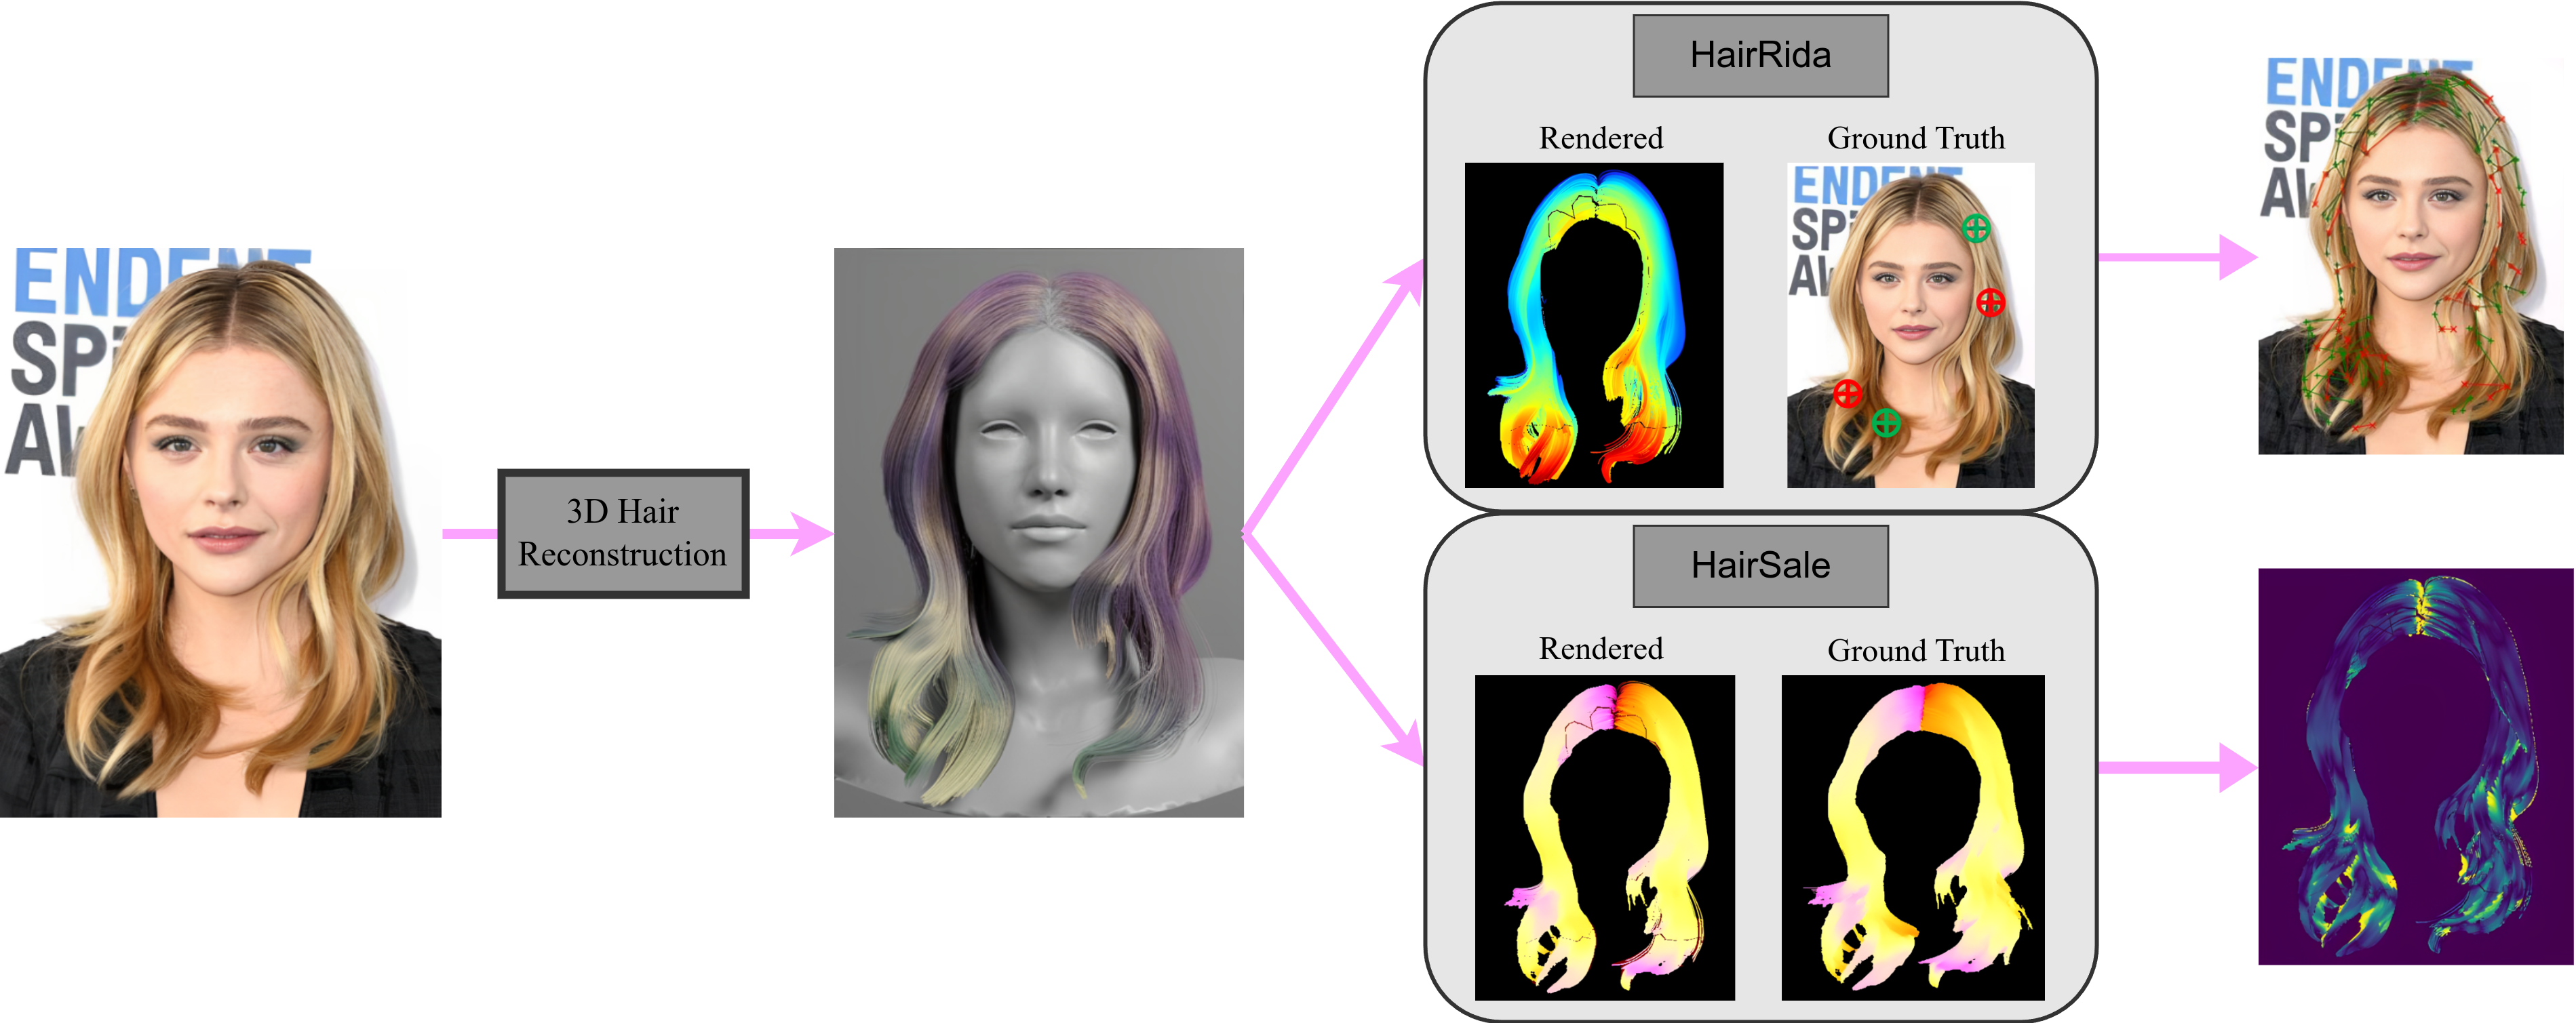
\includegraphics[width=0.95\textwidth]{assets/figures/eval/metrics/metrics.png}
        \caption{\textit{HairSale} and \textit{HairRida}.}
    \end{figure}
\end{frame}

\begin{frame}[t]{Datasets}
    \textbf{Synthetic: USC-HairSalon\cite{Hu2015SingleviewHM}}
    \begin{itemize}
        \item \textbf{343} 3D hair models, multiple views.
        \item \emph{HairStep} (strand + depth maps), ground-truth fields.
    \end{itemize}
    \vspace{5pt}
    \textbf{Real: \emph{HiSa} \& \emph{HiDa}}
    \begin{itemize}
        \item \textbf{1,250} portraits.
        \item \emph{HiSa}: 2D strand maps.
        \item \emph{HiDa}: Ordinal depth pairs.
        \item 80\% train, 20\% test.
    \end{itemize}
\end{frame}



\begin{frame}[t]{Quantitative Results: Synthetic}
    \textbf{Benchmarks: USC-HairSalon}
    \begin{itemize}
        \item \textbf{Baselines}:
        \begin{itemize}
            \item HairNet~\cite{zhou2018hairnet}, DynamicHair~\cite{yang2019dynamic}, NeuralHDHair~\cite{wu2022neuralhdhair}
        \end{itemize}
        \item \textbf{Occupancy Accuracy}:
        \begin{itemize}
            \item Ours: \(\uparrow\) 2-4\% improvement vs. baselines.
        \end{itemize}
        \item \textbf{Orientation Error}:
        \begin{itemize}
            \item Reduction by \(\sim\)10-20\% in angle or $\ell_2$ norm.
        \end{itemize}
    \end{itemize}
    \vspace{5pt}
    \textbf{Key Observation:} Strand+Depth input significantly outperforms orientation-only methods.
\end{frame}

% Slide 7: Quantitative Results (Real)
\begin{frame}[t]{Quantitative Results: Real}
    \textbf{Evaluations on \emph{HiSa} and \emph{HiDa}}
    \begin{itemize}
        \item \textbf{\emph{HairSale} (Strand Error)}:
        \begin{itemize}
            \item $\approx$ 16-18$^\circ$ error (ours) vs. 20$^\circ+$ (baselines).
        \end{itemize}
        \item \textbf{\emph{HairRida} (Depth Accuracy)}:
        \begin{itemize}
            \item Correct ordering rate: $\approx$75-78\% (ours), significantly better than others.
        \end{itemize}
        \item \textbf{Mask IoU}: 
        \begin{itemize}
            \item $\uparrow$ 1-3\% improvement on real images.
        \end{itemize}
    \end{itemize}
    \vspace{5pt}
    \textbf{Interpretation:} The hybrid strand+depth input plus domain adaptation narrows the real-synthetic gap.
\end{frame}

% Slide 8: Qualitative Results & Visualizations
\begin{frame}[t]{Qualitative Results \& Visualizations}
    \begin{itemize}
        \item \textbf{Synthetic Examples}:
        \begin{itemize}
            \item Overlay reconstructed strands vs. ground-truth. Observe alignment and geometry fidelity.
        \end{itemize}
        \item \textbf{Real Portraits}:
        \begin{itemize}
            \item Compare to baselines (e.g., orientation-only methods). Our results show sharper flow and consistent depth layering.
        \end{itemize}
        \item \textbf{User Study (Optional)}:
        \begin{itemize}
            \item Approximately 60\% of participants prefer our outputs over baselines.
        \end{itemize}
    \end{itemize}
\end{frame}

% Slide 9: Ablation Studies
\begin{frame}[t]{Ablation Studies}
    \begin{itemize}
        \item \textbf{Strand Map vs. Filtered Orientation}:
        \begin{itemize}
            \item Strand map reduces noise, clarifies direction (up to 20\% angle improvement).
        \end{itemize}
        \item \textbf{Depth Map Contribution}:
        \begin{itemize}
            \item Removing depth reduces geometry accuracy; domain adaptation with pseudo labels crucial for real data.
        \end{itemize}
        \item \textbf{Loss Functions}:
        \begin{itemize}
            \item Full $L_{\mathrm{occ}} + L_{\mathrm{orient}}$ performs best; dropping orientation leads to inconsistent hair growth.
        \end{itemize}
    \end{itemize}
\end{frame}

% Slide 10: Limitations & Future Directions
\begin{frame}[t]{Limitations \& Future Directions}
    \begin{itemize}
        \item \textbf{Rare Hairstyles}:
        \begin{itemize}
            \item Braids, extreme curls not well-represented in synthetic data; reconstructions can fail.
        \end{itemize}
        \item \textbf{Annotation Cost}:
        \begin{itemize}
            \item Dense strand annotation is time-intensive for \emph{HiSa}.
        \end{itemize}
        \item \textbf{Ordinal Depth Ambiguity}:
        \begin{itemize}
            \item Relative depth (in \emph{HiDa}) is weaker than full ground-truth; certain 3D details may remain ambiguous.
        \end{itemize}
        \item \textbf{Future Work}:
        \begin{itemize}
            \item More diverse synthetic hair datasets, semi-supervised annotation, multi-view expansions.
        \end{itemize}
    \end{itemize}
\end{frame}
